\documentclass[12pt,journal]{IEEEtran}
\usepackage[letterpaper, margin=0.8in]{geometry}
\usepackage{framed, listings, graphicx, float, amsmath}

\begin{document}

\title{
\includegraphics[width=0.4\linewidth]{figures/rewrite}}

\author{EE149/249A Project Report, Fall 2015

Reia Cho, CJ Geering, Nathaniel Mailoa, Rachel Zhang

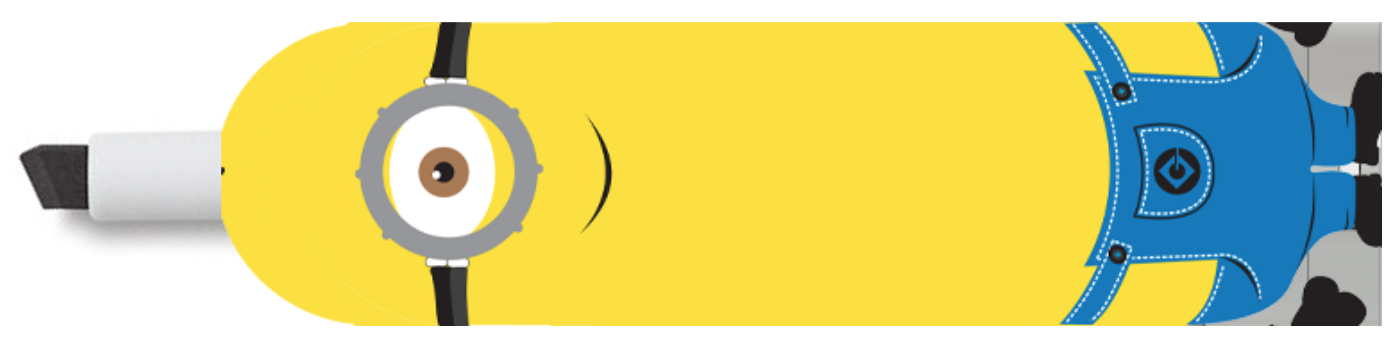
\includegraphics[width=0.45\linewidth]{figures/minion}}


% make the title area
\maketitle



\section{Introduction}
INSERT TEXT HERE

\section{Bill of Materials}
\centering
\begin{tabular}{r|l}
Component & Price \\
\hline
LightBlue Bean & \$30 \\
BNO055 Absolute Orientation Sensor & \$35 \\
Li-Ion 3.7V 150mAh Battery and Charger & \$13 \\
Force Sensor & \$7 \\
Button and LED & \$2 \\
3D Printing & \$2 \\
\hline
Total & \$89 \\
\end{tabular}

\section{System}

\begin{figure}[H]
  \centering
    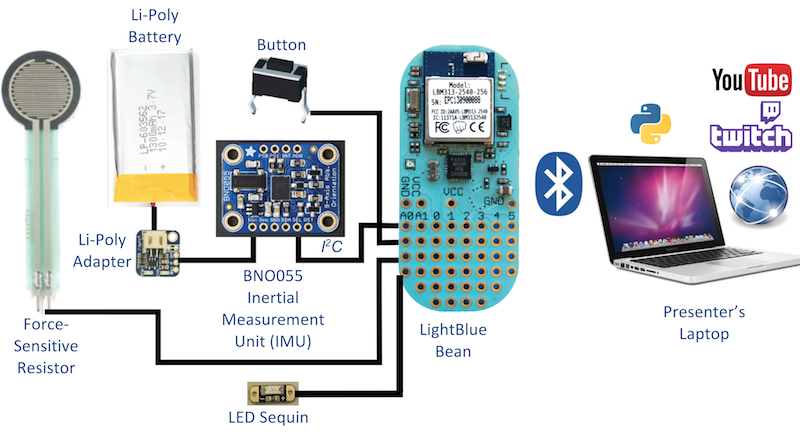
\includegraphics[width=\linewidth]{figures/system}
  \caption{reWRITE system}
  \label{fig:system}
\end{figure}

INSERT TEXT HERE

\subsection{LightBlue Bean}

\begin{figure}[H]
  \centering
    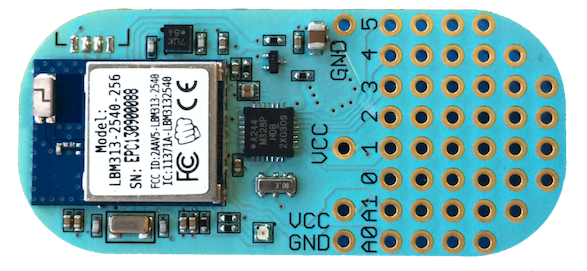
\includegraphics[width=0.8\linewidth]{figures/bean}
  \caption{LightBlue Bean}
  \label{fig:bean}
\end{figure}

INSERT TEXT HERE

\subsection{BNO055 Absolute Orientation Sensor Breakout Board}

\begin{figure}[H]
  \centering
    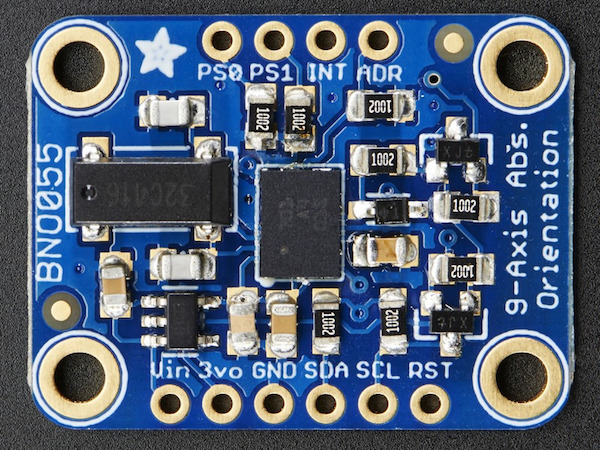
\includegraphics[width=0.6\linewidth]{figures/imu}
  \caption{BNO055 IMU breakout board}
  \label{fig:imu}
\end{figure}

INSERT TEXT HERE

\subsection{Li-Ion Battery}

\begin{figure}[H]
  \centering
    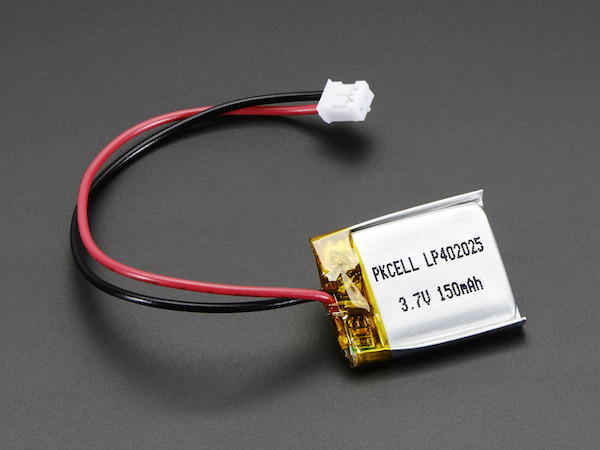
\includegraphics[width=0.6\linewidth]{figures/battery}
  \caption{3.7V 150mAh Li-Ion battery}
  \label{fig:battery}
\end{figure}

INSERT TEXT HERE

\subsection{Force Sensor}

\begin{figure}[H]
  \centering
    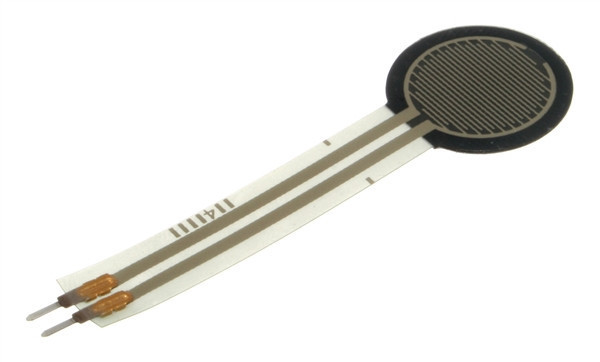
\includegraphics[width=0.6\linewidth]{figures/force-sensor}
  \caption{Force sensor}
  \label{fig:system}
\end{figure}

INSERT TEXT HERE

\subsection{Button and LED Sequin}
INSERT TEXT HERE

\section{Casing}
INSERT TEXT HERE

\begin{figure}[h]
  \centering
    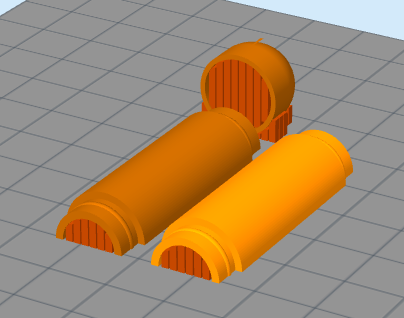
\includegraphics[width=0.6\linewidth]{figures/3d-model}
  \caption{Casing model}
  \label{fig:3d-model}
\end{figure}

\begin{figure}[h]
  \centering
    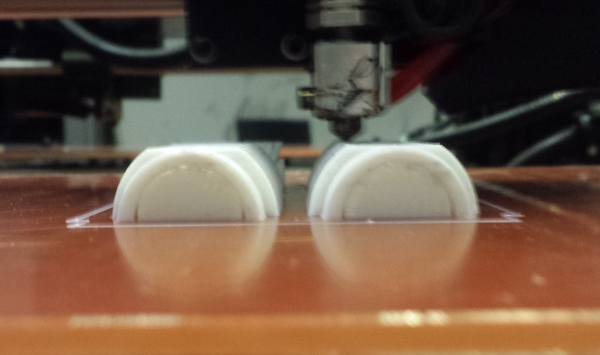
\includegraphics[width=0.6\linewidth]{figures/3d-print}
  \caption{3D printing the casing}
  \label{fig:3d-print}
\end{figure}

\section{Position Reconstruction}
INSERT TEXT HERE

\subsection{IMU Sensor Data}
INSERT TEXT HERE

\subsection{Filtering and Thresholding}
INSERT TEXT HERE

\begin{figure}[h]
  \centering
    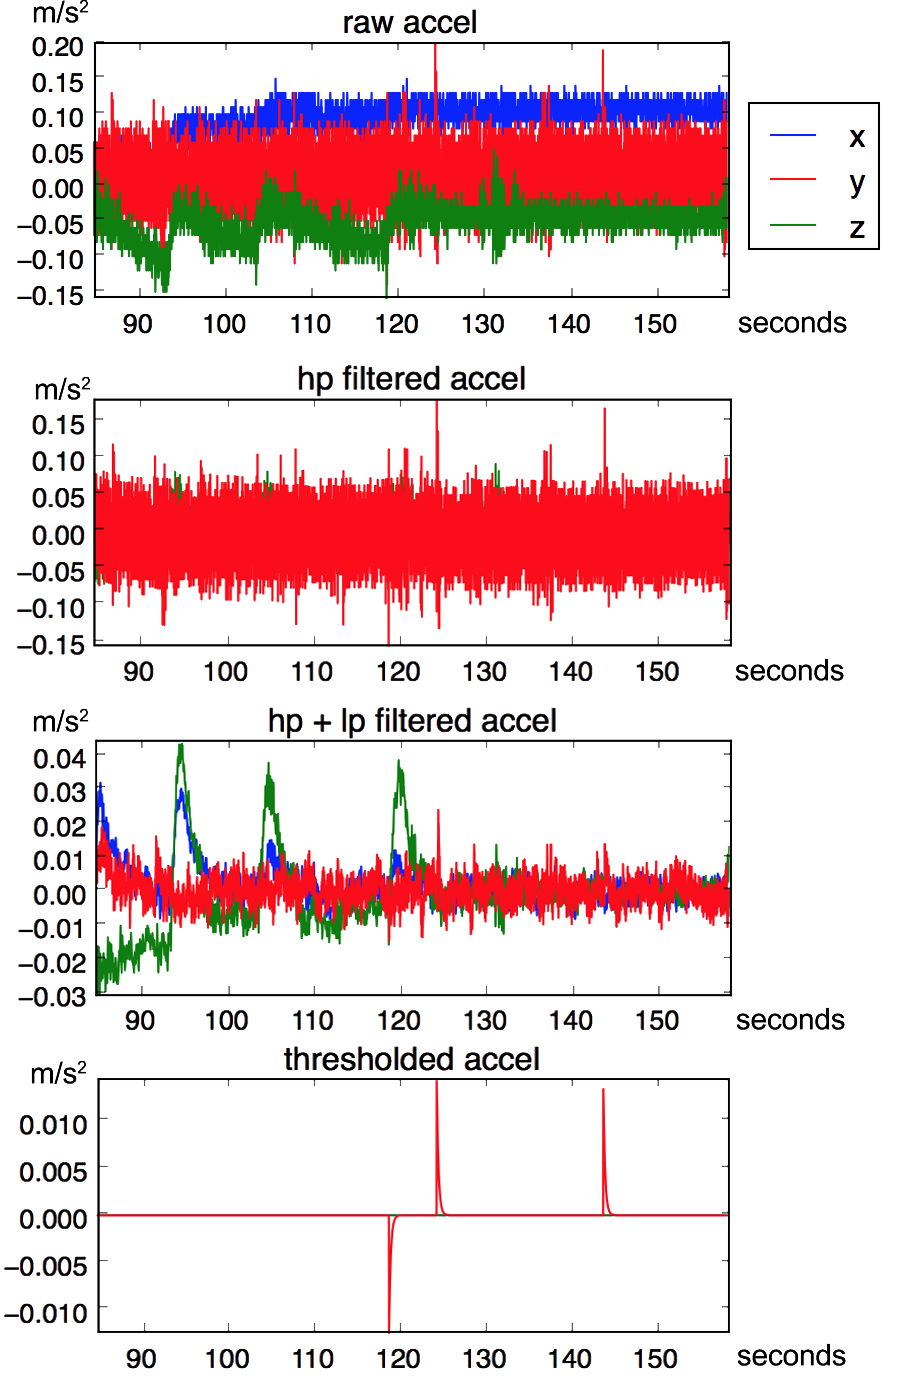
\includegraphics[width=\linewidth]{figures/filtering}
  \caption{(a) Raw data from IMU; (b) Processed with high pass filter; (c) Processed with low pass filter; (d) Thresholded}
  \label{fig:filtering}
\end{figure}

\subsection{Transformation to Fixed Reference Frame}
INSERT TEXT HERE

\begin{figure}[h]
  \centering
    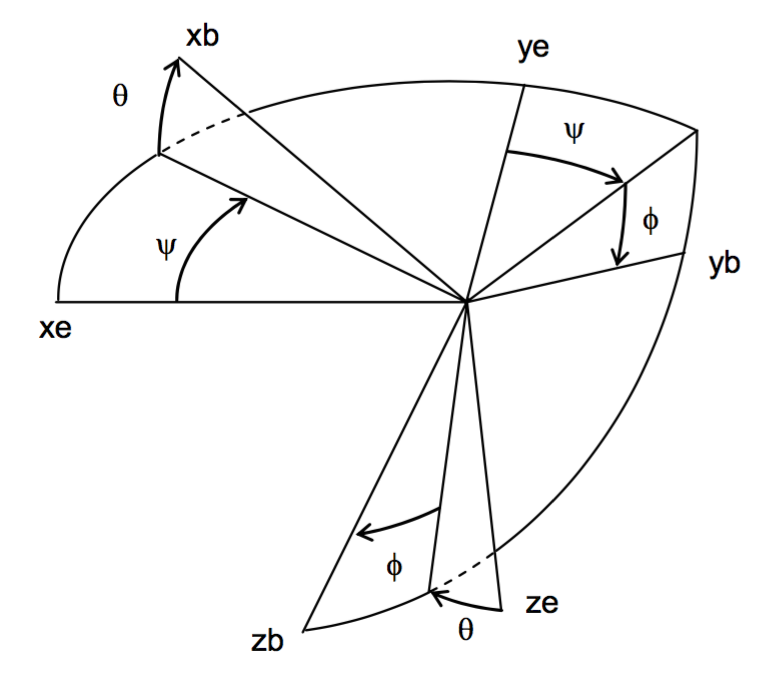
\includegraphics[width=\linewidth]{figures/dcm}
  \caption{Angles corresponding to the DCM [Premerlani and Bizard]}
  \label{fig:vel-adjust}
\end{figure}

\subsection{Velocity Adjustment}
INSERT TEXT HERE
$$v_{\text{adjusted}}[n] = v_{\text{unadjusted}}[n] - \left(\frac{n-i}{j-i}\right)^2 v_{\text{unadjusted}}[j]$$

\begin{figure}[h]
  \centering
    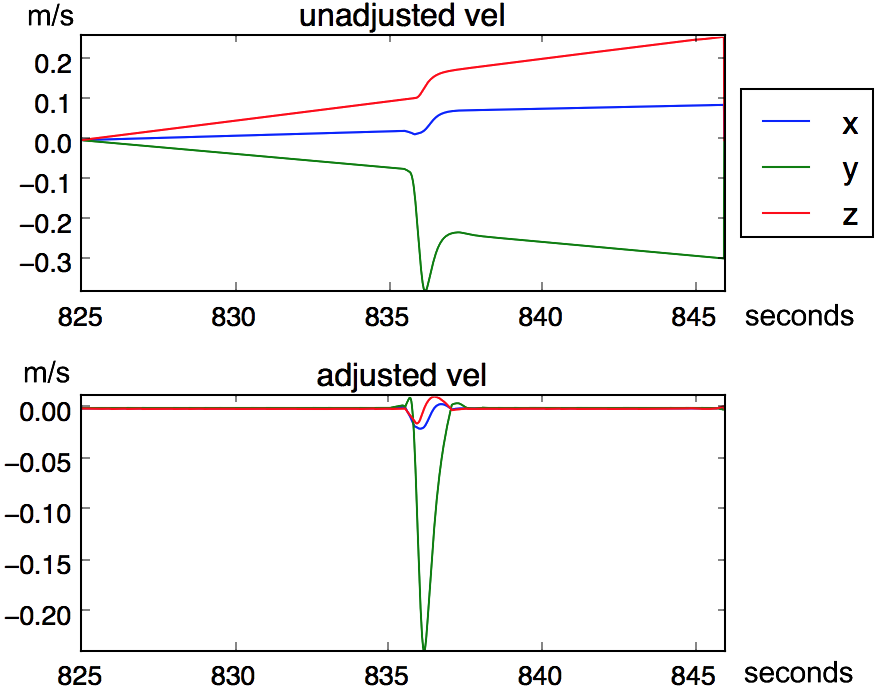
\includegraphics[width=\linewidth]{figures/vel-adjust}
  \caption{(a) Velocity integrated from acceleration data; (b) After velocity adjustment}
  \label{fig:vel-adjust}
\end{figure}

\subsection{Tip Position Reconstruction}
INSERT TEXT HERE


\subsection{Plotting}
INSERT TEXT HERE

\section{Quantitative Analysis and Scheduling}
INSERT TEXT HERE

\section{Mode of Operation}
INSERT TEXT HERE

\section{Acknowledgements}
We would like to acknowledge the following individuals for their support and contribution in this project.
\begin{itemize}
\item Trung Tran, \textit{National Instruments}
\item Prof. Sanjit Seshia, \textit{UC Berkeley}
\item Matthew Weber, \textit{UC Berkeley}
\item Eric Kim, \textit{UC Berkeley}
\item Casey Rogers, \textit{UC Berkeley 3D Modeling Club}
\end{itemize}

\begin{thebibliography}{1}
\bibitem{PB} Premerlani, W., Bizard, P.: Direction cosine matrix	IMU: theory. http://gentlenav.googlecode.com/files/DCMDraft2.pdf
\end{thebibliography}

\newpage
\onecolumn

\section{Appendix 1: LightBlue Bean code}
\small{
\lstinputlisting[language=C,frame=single,breaklines=true]{stream_data.ino}
}

\section{Appendix 2: Python code}
\small{
\lstinputlisting[language=Python,frame=single,breaklines=true]{draw.py}
}

\end{document}



